\documentclass[11pt]{article}

\usepackage[a4paper,margin=27mm]{geometry}
\usepackage[T1]{fontenc}
\usepackage[utf8]{inputenc}
\usepackage{newtxtext}
\usepackage[amsthm]{newtxmath}
\usepackage{microtype}
\usepackage{booktabs}
\usepackage{graphicx}
\usepackage{flafter}
\usepackage[section]{placeins}
\usepackage{caption}
\usepackage{enumitem}
\usepackage{xcolor}
\usepackage[hidelinks]{hyperref}

\captionsetup{font=small,labelfont=bf}
\setlist[itemize]{leftmargin=*,topsep=4pt,itemsep=2pt}
\setlist[enumerate]{leftmargin=*,topsep=4pt,itemsep=3pt}
\setlength{\parindent}{1.2em}
\setlength{\parskip}{0pt}

\newtheorem{definition}{Definition}
\newtheorem{proposition}{Proposition}
\newtheorem{lemma}{Lemma}
\newtheorem{theorem}{Theorem}

\newcommand{\argine}{\textsc{Argine}}
\newcommand{\ews}{\mathrm{EWS}}
\newcommand{\budget}{M}
\newcommand{\footprint}{F}

\title{\textbf{Argine: Expert Streaming Under Hard Memory Constraints}\\
\large Allocation, Selection, and Performance Regimes in Mixture-of-Experts Inference}
\author{sennape}
\date{October 2026}

\begin{document}

\maketitle

\begin{abstract}
Mixture-of-experts (MoE) models decouple total parameter count from per-token computation, but under hard DRAM limits their inactive parameters do not disappear: non-resident expert weights must be fetched, retained, and evicted under a dynamically changing routing workload. We study CPU-only expert streaming from NVMe across two MoE models, multiple workloads, and memory-pressure regimes. Expert working sets are heterogeneous across layers, and uniform per-layer memory partitioning is measurably suboptimal in the evaluated replay traces. The tested layer-aware allocation improves cache effectiveness under pressure, yet the remaining future-informed expert-selection headroom is substantially larger than the gain obtained from reallocation alone. Routing distributions change strongly across workload boundaries, but a fixed allocation equal to the tested controller's mean allocation explains most or all of its gain, falsifying the temporal mechanism of that controller without implying that dynamic adaptation is ineffective in general. An interpretable latency decomposition predicts measured 30B token latency with a median leave-one-configuration-out absolute percentage error of 2.25\%. Finally, extreme-pressure experiments show that the one-token expert footprint is not a hard execution threshold, and a preregistered matched-pressure experiment does not reproduce the historical cross-model regime difference. These results support treating expert residency as a joint allocation-and-retention problem rather than reducing it to cache capacity or conventional hit rate alone.
\end{abstract}

\section{Introduction}
\label{sec:introduction}

Mixture-of-experts (MoE) architectures increase model capacity by activating only a subset of experts for each token. This conditional computation changes the memory problem, but it does not remove it. When the complete expert set does not fit in DRAM, inference must decide which expert weights remain resident, which are evicted, and which non-resident experts are fetched from secondary storage. Under a hard expert-memory budget, these decisions interact with routing, I/O concurrency, and the temporal structure of the workload.

A natural first abstraction is \emph{residency}: performance should improve as a larger fraction of the expert weights fits in memory. Our measurements show that this view is incomplete. Equal-sized layers do not exhibit equal working-set demand. The same number of misses can imply different stall time because reads overlap differently at different queue depths. Routing distributions can drift across workload boundaries without a controller obtaining useful gain from reacting quickly to that drift. Moreover, historical pressure-response differences observed across models and binaries in different pressure regions need not reproduce in a matched-$M/F$ comparison on the current runtime.

This paper studies that gap between nominal residency and realized performance. We use \argine{}, an experimental framework for CPU-only MoE inference with expert weights streamed from NVMe under an explicit DRAM cap. The goal is not to present a universal production memory manager. Instead, we use controlled replay, end-to-end execution, preregistered experiments, and negative results to isolate which parts of the problem are explained by layer allocation, which remain attributable to expert selection and I/O behavior, and which apparently simple performance abstractions fail under stronger pressure.

\subsection{From cache capacity to allocation and retention}

Let $\budget$ denote the DRAM budget available to resident expert weights. A conventional cache-capacity view asks whether the total resident fraction is large enough and which objects should be evicted on a miss. MoE inference introduces an additional structure: expert demand is partitioned by layer, and a token visits these layers in a fixed computational order while router decisions determine which experts are required within each layer. The memory manager therefore faces at least two coupled decisions:
\begin{enumerate}
    \item \emph{allocation}: how much of $\budget$ to assign to each layer; and
    \item \emph{retention}: which experts to keep within each layer's allocation.
\end{enumerate}

This distinction matters empirically. If layer working sets differ, a uniform split can waste capacity even when total memory is fixed. Conversely, improving the split does not solve the entire problem if the dominant remaining misses arise from poor expert selection within the allocated space. We therefore separate the value of layer-aware allocation from the residual headroom exposed by a future-informed selection reference.

\subsection{Why hit rate is not enough}

Hit rate is useful for describing reuse, but it is not itself a time model. In the evaluated runtime, expert-level reuse and runtime-style hit accounting are distinct quantities, and miss count does not map linearly to stall time. As memory pressure rises, more misses can increase I/O queue depth and overlap, reducing the average time attributable to each individual read. A policy that prevents more misses can therefore save less wall-clock time than a simple hit-rate comparison suggests.

This motivates a second question: can measured token latency be explained by a decomposition that explicitly represents unhidden I/O rather than by miss count alone? We test an interpretable model of token time and evaluate it out of configuration rather than only by in-sample fit.

\subsection{Pressure regimes and mechanism tests}

A further temptation is to normalize memory by a model-specific footprint and treat the resulting ratio as a universal pressure coordinate. We use the one-token expert footprint $\footprint$ as such a scale and study $\budget/\footprint$ down to regimes where expert reuse nearly vanishes. The resulting measurements separate three notions that are often conflated: reuse collapse, degraded but continuing execution, and hard non-completion. We then compare two MoE models at matched $\budget/\footprint$ to test whether a previously observed cross-model difference in pressure response reproduces under a controlled matched-pressure protocol.

The answer is deliberately mixed. Some structural effects reproduce strongly: layer demand is heterogeneous, uniform allocation is suboptimal, and workload boundaries exhibit substantial routing drift. Other hypotheses do not survive direct tests: the tested adaptive controller does not obtain its gain from rapid temporal reaction, and the historical cross-model pressure-regime difference is not distinguished in the matched-pressure experiment on the current runtime. We retain these negative and inconclusive outcomes because they constrain the design space as much as the positive results do.

\subsection{Contributions}

The paper makes six empirical and methodological contributions:
\begin{enumerate}
    \item \textbf{Layer heterogeneity.} We quantify per-layer expert working sets across two MoE models and show that a uniform per-layer memory split is measurably suboptimal in the evaluated traces.
    \item \textbf{Allocation versus selection.} We show that layer-aware allocation becomes increasingly valuable under memory pressure, while the remaining future-informed expert-selection headroom is substantially larger than the allocation gain.
    \item \textbf{Temporal adaptation.} We measure strong routing-distribution drift at workload boundaries but falsify the temporal mechanism of the current \texttt{adaptive-e64} controller: a fixed allocation equal to its mean allocation explains most or all of the observed gain.
    \item \textbf{Metric semantics.} We separate expert-level reuse from runtime-style hit accounting and show why miss count alone is insufficient to model elapsed time under changing I/O concurrency.
    \item \textbf{Interpretable latency prediction.} A decomposition of token latency into compute, unhidden I/O, synchronization, and controller components achieves a median leave-one-configuration-out absolute percentage error of 2.25\% on the preregistered 30B primary test; the decomposition is predictive rather than component-identifying.
    \item \textbf{Pressure-regime limits.} Extreme-pressure experiments show that the one-token expert footprint is not a hard execution threshold, and a preregistered matched-pressure experiment does not reproduce the historical cross-model regime difference.
\end{enumerate}

Together, these results support a more cautious systems abstraction: expert residency under hard memory constraints should be treated as a coupled allocation-and-retention problem whose performance is mediated by routing structure, selection quality, and I/O concurrency. We do not claim that this settles the general theory of MoE memory management; rather, it identifies which simpler abstractions fail in the evaluated regimes and where the largest measured optimization headroom remains.

\section{System Model and Problem Formulation}
\label{sec:system-model}

\begin{figure}[t]
    \centering
    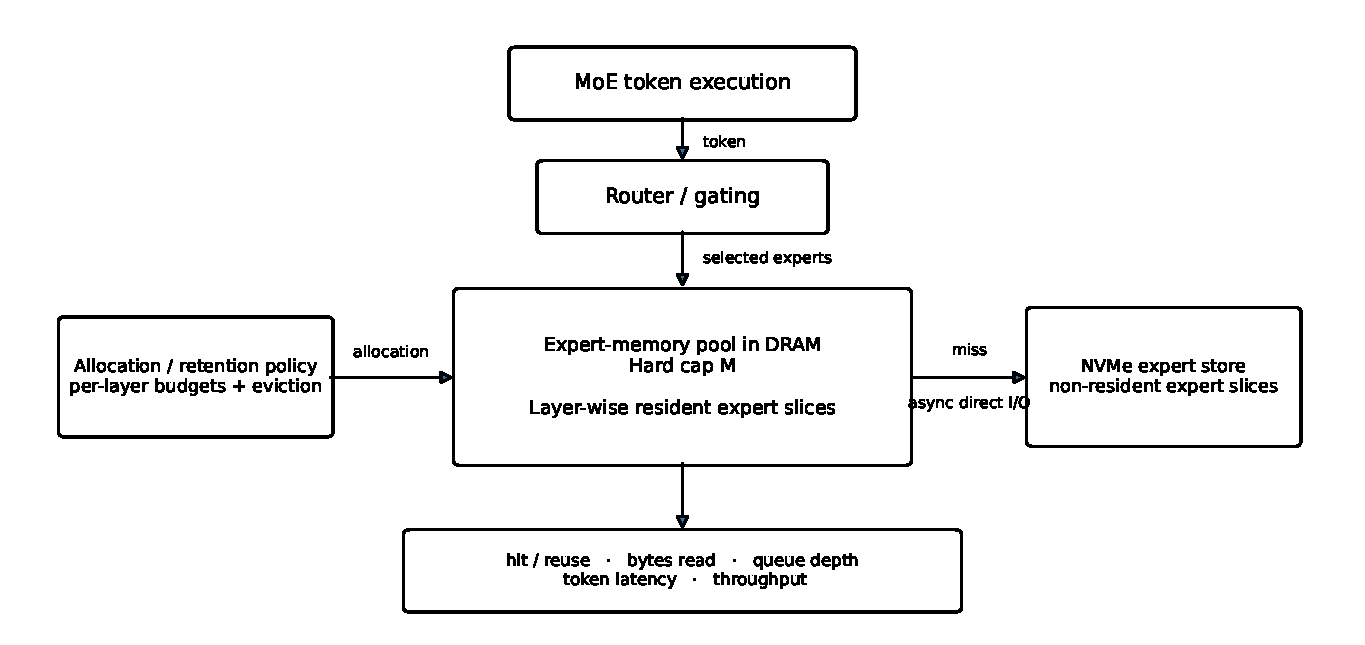
\includegraphics[width=0.96\linewidth]{../docs/figures/argine_system_architecture.pdf}
    \caption{Expert streaming under a hard DRAM budget. For each token, the router selects experts whose weights must reside in a bounded DRAM expert-memory pool. The allocation/retention policy determines per-layer memory budgets and eviction decisions. Requests for non-resident experts trigger asynchronous direct reads from the NVMe expert store. The experiments characterize this coupled allocation-and-retention process through reuse, I/O volume, queue depth, token latency, and generation throughput.}
    \label{fig:architecture}
\end{figure}

\subsection{Expert streaming under a hard memory budget}

We consider autoregressive inference for a sparse mixture-of-experts model with $L$ MoE layers. At layer $l$, a router selects a subset of experts for the current token. Expert weights are stored on NVMe and may be resident in a bounded DRAM pool. Non-expert weights remain resident and are outside the expert-memory budget considered here. Figure~\ref{fig:architecture} summarizes the resulting data path.

\begin{definition}[Expert-memory budget]
The expert-memory budget $M$ is the maximum DRAM capacity available to resident expert weights. It is a hard ceiling enforced by the expert store and is distinct from the memory occupied by non-expert model state, the KV cache, runtime buffers, and the operating system.
\end{definition}

The runtime partitions the expert store into shards, and residency is ultimately enforced at slice granularity. A requested expert is usable only when the required slices can be made resident and pinned for the corresponding computation. A miss therefore triggers storage activity before the dependent computation can proceed. This makes the observed token time a function not only of how much expert memory is resident, but also of which experts are retained and how concurrent I/O requests overlap.

\subsection{Allocation and retention}

Let $M_l$ denote the expert-memory budget assigned to layer $l$. A feasible layer allocation satisfies
\begin{equation}
    M_l \geq 0,
    \qquad
    \sum_{l=1}^{L} M_l \leq M .
    \label{eq:allocation-budget}
\end{equation}
The \emph{allocation} problem chooses the vector
\begin{equation}
    \mathbf{M}=(M_1,\ldots,M_L),
    \label{eq:allocation-vector}
\end{equation}
whereas the \emph{retention} problem chooses which expert slices occupy the capacity assigned to each layer. These are coupled but distinct decisions. Reallocating memory can reduce misses caused by an unfavorable partition even if the replacement rule within a layer is unchanged; conversely, an improved partition cannot remove misses caused by poor retention within the allocated capacity.

This separation motivates the principal policy comparison used later in the paper. Global LRU supplies a conventional recency baseline. Per-layer uniform LRU isolates the effect of partitioning memory equally across layers. The tested \texttt{adaptive-e64} policy changes layer allocations in replay. A Belady-style future-informed reference supplies a deliberately unattainable comparison that quantifies residual selection headroom rather than an implementable online policy.

\subsection{Expert working sets}

For a layer $l$ and a routing trace $W$, let $p_{l,e}(W)$ be the observed fraction of routed selections assigned to expert $e$. Sort experts in decreasing order of $p_{l,e}$. For a coverage target $q\in(0,1)$, define the effective expert working set
\begin{equation}
    \mathrm{EWS}_{q}(l,W)
    =
    \min\left\{
        k:
        \sum_{e=1}^{k} p_{l,(e)}(W) \geq q
    \right\},
    \label{eq:ews}
\end{equation}
where $p_{l,(e)}$ denotes the $e$th largest routing frequency. We report both the expert count and its normalized form
\begin{equation}
    f_{q,l}(W)
    =
    \frac{\mathrm{EWS}_{q}(l,W)}{N_l},
    \label{eq:ews-fraction}
\end{equation}
with $N_l$ the number of routed experts in layer $l$. Section~\ref{sec:heterogeneity} uses $q=0.90$ to characterize layer heterogeneity.

EWS is a demand descriptor, not a cache model. It summarizes concentration over an observed trace but does not encode temporal order, co-activation, expert size, sharding, or I/O overlap. We therefore treat it as one explanatory variable rather than as a sufficient predictor of performance.

\subsection{Normalized pressure and one-token footprint}

To compare memory pressure across the two evaluated models, we define a model-specific one-token expert footprint $F$. For each MoE layer, the router selects $k_l$ routed experts. Let $s_{l,e}$ be the expert-store bytes required for one expert of that layer, including the gate, up, and down slices after the store's alignment rule. Then
\begin{equation}
    F
    =
    \sum_{l=1}^{L} k_l s_l ,
    \label{eq:footprint}
\end{equation}
where $s_l$ is the per-expert stored size for layer $l$. The 80B model's shared expert is not part of the expert store and is therefore excluded from $F$.

For the evaluated quantized models, the derived footprints are
\begin{equation}
    F_{30}=1{,}097{,}072{,}640~\mathrm{B}
    \approx 1.0217~\mathrm{GiB},
    \qquad
    F_{80}=719{,}585{,}280~\mathrm{B}
    \approx 0.6702~\mathrm{GiB}.
    \label{eq:footprints}
\end{equation}
We use
\begin{equation}
    \rho = \frac{M}{F}
    \label{eq:normalized-pressure}
\end{equation}
as a physically motivated pressure coordinate in the extreme-pressure and matched-pressure experiments. Importantly, $F$ is a derived scale, not a claimed feasibility threshold. Section~\ref{sec:pressure-regimes} directly tests that distinction.

\subsection{Metrics and performance quantities}

We distinguish three classes of measurements.

\paragraph{Reuse.}
Expert-level reuse describes whether the expert demand represented by a routing event is already resident under the relevant replay or diagnostic semantics. Runtime-style hit accounting instead follows the expert store's slice-level bookkeeping. The two quantities are related but not interchangeable.

\paragraph{I/O.}
We record bytes read, read count, and queue-depth information. Queue depth matters because misses can overlap: the wall-clock cost of an additional miss depends on how much of its I/O is hidden behind other reads or computation.

\paragraph{End-to-end performance.}
The principal runtime quantities are generation throughput in tokens/s and its reciprocal token latency in ms/token. Time-to-first-token and prompt throughput are reported where relevant but are not the primary optimization target in the results presented here.

The central systems question can therefore be stated more precisely than ``how much of the model fits in memory'': given a hard expert-memory budget $M$, how should memory be allocated across layers and retained within those allocations so as to minimize the \emph{time cost} of non-resident expert demand?

\section{Experimental Methodology}
\label{sec:methodology}

\subsection{Reference platform}

All measurements in this paper were collected on one controlled consumer machine; hardware generalization is therefore outside the scope of the empirical claims. The reference system uses an Intel Core i5-1340P with four performance cores, eight efficiency cores, 16 logical CPUs, and AVX2 support; 16\,GB of RAM (15.72\,GiB usable); NVMe storage; integrated Intel Iris Xe graphics; and Windows~11. All reported model execution uses the CPU backend with zero GPU layers.

The expert-store runtime is a patched \texttt{llama.cpp}~\cite{gerganov2023llamacpp}. The current research binary used by the later confirmatory experiments is based on \texttt{llama.cpp} commit \texttt{254b177} with the Argine expert-store and research instrumentation. It uses asynchronous direct I/O, bypassing the operating-system file cache on the measured expert-store path. Unless an experiment explicitly states otherwise, the later frozen configuration uses context size 4096, batch size 2048, micro-batch size 512, f16 KV storage, flash attention enabled, and pretouch disabled.

The repository retains historical binary provenance because the binary itself is an experimental variable. The EXP-007 characterization campaign spans the validated trace formats used during its collection; later controlled experiments use the current \texttt{llama-research-v2} runtime. We do not pool timings across binaries unless the corresponding experiment explicitly licenses that comparison.

\subsection{Models}

Table~\ref{tab:models} summarizes the two experimental regimes. We refer to them as 30B and 80B for brevity, but do not interpret them simply as ``small'' and ``large'': architecture, expert count, quantization, slice sizes, and active parameter count all differ.

\begin{table}[t]
    \centering
    \caption{Evaluated MoE models. Expert and non-expert byte counts are those recorded by the Argine artifact for the quantized GGUFs used in the experiments.}
    \label{tab:models}
    \small
    \begin{tabular}{lcc}
        \toprule
        & \textbf{30B} & \textbf{80B} \\
        \midrule
        Model & Qwen3-30B-A3B~\cite{qwen3technicalreport} & Qwen3-Next-80B-A3B-Instruct~\cite{qwen3next2025} \\
        Total / active parameters & 30.5B / 3.35B & 79.7B / 3.87B \\
        MoE layers & 48 & 48 \\
        Routed experts / layer & 128 & 512 \\
        Active routed experts / token & 8 & 10 \\
        Quantization & Q4\_K\_M & Q3\_K\_M \\
        Expert bytes & 16.35\,GiB & 34.31\,GiB \\
        Non-expert bytes & $\sim$1.0\,GiB & 1.35\,GiB \\
        One-token footprint $F$ & 1.0217\,GiB & 0.6702\,GiB \\
        \bottomrule
    \end{tabular}
\end{table}

The 80B architecture also contains a shared expert that is not managed by the expert store; it is excluded from the routed-expert footprint defined in Eq.~\eqref{eq:footprint}. At a 4\,GiB expert-memory budget, the nominal expert-byte residency is approximately 24.5\% for the 30B and 11.7\% for the 80B, illustrating why raw resident fraction is not directly comparable to active demand.

\subsection{Workloads and splits}

The main routing characterization uses seven workload families: natural language, coding, reasoning/math, structured JSON, Italian, multi-turn, and transition traces. Where a workload has DEV/EVAL splits, DEV is used for tuning or hypothesis formation and EVAL for held-out or retrospective evaluation according to the protocol of the corresponding experiment.

EXP-007 closes a $2\times 7\times 2$ characterization grid: two models, seven workload families, and DEV/EVAL, for 28 cells. Each cell is evaluated at the relevant memory budgets, and the closed characterization retains three replay-qualified runs per cell-budget. Transition traces concatenate qualitatively different segments and are used separately to study temporal drift rather than being treated as another stationary workload.

Later performance experiments use frozen prompts or workload files specified by their protocols. In particular, the extreme-pressure performance arm uses an unchanged benchmark prompt with 128 generated tokens per measured request, while its diagnostic arm uses the natural-language EVAL workload. The replication unit for performance experiments is a fresh complete launch rather than an individual token.

\subsection{Tracing and event-atomic replay}

Argine records expert-routing and expert-store events without allowing the instrumentation to control the policy. Replay operates on \emph{events}: the set of experts required together by one forward-pass MoE node. The runtime pins the slices required by the current node; replay therefore treats the event as atomic and does not permit a policy to evict a member of the event while it is being served.

Replay fidelity was validated separately before policy conclusions were drawn. Under the qualified conditions, the replay reproduces the expert-store decisions required for the reported counterfactual comparisons. This qualification is essential because the runtime caches address-keyed slices rather than idealized whole experts, and a replay that ignores pins, sharding, or slice granularity can overstate achievable hit rates.

Instrumentation overhead was also measured separately. At the 4\,GiB configuration, the measured 95\% confidence interval lies entirely below 2\%; at 1.5\,GiB the result is inconclusive. Accordingly, traced data are used for routing and mechanism claims, while the strongest performance claims rely on the untraced performance blocks specified by their experiments.

\subsection{Policy comparisons}

The replay experiments compare policies at a fixed total expert-memory budget. The key references used in this paper are:
\begin{itemize}
    \item \textbf{global LRU}, a conventional global recency baseline;
    \item \textbf{per-layer uniform LRU}, which partitions the budget equally across layers and applies recency within each partition;
    \item \textbf{\texttt{adaptive-e64}}, the tested layer-aware controller used in the final replay analysis; and
    \item \textbf{Belady-style future-informed selection}, an offline reference that uses future information and is therefore not an implementable online policy.
\end{itemize}

The Belady-style reference is included to estimate residual selection opportunity, not to claim an achievable runtime speedup. Likewise, the adaptive controller exists in replay only in the experiments reported here; the paper does not present a runtime implementation of dynamic layer allocation.

\subsection{Memory-pressure experiments}

Three experimental designs supply the performance evidence used later in the paper.

\paragraph{Extreme pressure.}
The 30B primary arm evaluates 1.5\,GiB, 1152\,MiB, 1024\,MiB, 768\,MiB, and 512\,MiB. The 80B exploratory arm evaluates 1.5\,GiB, 768\,MiB, 672\,MiB, and 512\,MiB. Budgets are rotated across three rounds to reduce simple order effects. The principal performance outcome is generation tokens/s from an untraced launch. Separate diagnostic launches measure expert-level reuse. Budgets below 512\,MiB are excluded from the main arm because the expert-store shard count would change, introducing a second structural variable.

\paragraph{Interpretable performance model.}
The 30B performance-model experiment uses five memory configurations spanning 1.5\,GiB to 512\,MiB. The preregistered primary test is leave-one-configuration-out prediction error rather than in-sample fit. The model is
\begin{equation}
    T_{\mathrm{token}}
    =
    T_{\mathrm{compute}}
    +
    T_{\mathrm{unhidden\,I/O}}
    +
    T_{\mathrm{sync}}
    +
    T_{\mathrm{controller}} .
    \label{eq:latency-model}
\end{equation}
The design tests predictive usefulness of this decomposition; it does not guarantee separate causal identification of each fitted component.

\paragraph{Matched-pressure cross-model test.}
The final cross-model experiment fixes generation threads at four for both models and matches memory pressure using $\rho=M/F$. Three pressure points are measured with three complete launches per cell. The preregistered primary explanandum compares the P1$\rightarrow$P2 pressure-response exponent; P3 is secondary. This design was introduced specifically because the historical cross-model observations compared different normalized pressure regions on earlier binaries.

\subsection{Measurement semantics}

The paper keeps metric definitions tied to the mechanism that produces them.

\paragraph{Expert-level diagnostic hit rate.}
For the extreme-pressure diagnostic experiment, this is the workload gate-slice hit rate: slice hits divided by slice accesses in the first gate \texttt{MUL\_MAT\_ID} node of each layer, over prefill and decode, excluding warm-up and the flush sentinel.

\paragraph{Runtime-style hit rate.}
This follows the store's lower-level accounting and therefore reflects the slice-granular runtime rather than a whole-expert abstraction. The distinction is preserved throughout the paper instead of collapsing both quantities into a generic ``hit rate.''

\paragraph{Throughput and latency.}
Generation throughput is measured in tokens/s. Token latency is reported in ms/token and is the primary response for the interpretable performance model. Queue depth, reads/token, bytes/token, time-to-first-token, and prompt throughput are secondary mechanism or diagnostic quantities where relevant.

\subsection{Experimental discipline}

The research artifact uses permanent experiment identifiers, frozen protocols for confirmatory tests, explicit success or falsification criteria where applicable, and versioned analysis outputs. New criteria are not introduced after inspecting an outcome. When a preregistered test lacks a positive support threshold, a result may be ``not falsified by this test'' while the experiment remains formally inconclusive.

Negative results are retained rather than reinterpreted. In particular, the workload-drift experiment distinguishes positive descriptive evidence of routing drift from the falsified claim that the tested controller shortens the transition transient. Likewise, failure to reproduce the historical 30B/80B regime difference in the matched-pressure experiment does not rewrite measurements from earlier binaries and pressure regions.

The repository distinguishes \emph{measured} quantities read from run artifacts, \emph{derived} quantities computed by declared analyses, hypotheses, supported or falsified tests, open questions, and limitations. This separation is part of the methodology: the paper's claims are restricted to the scope licensed by the corresponding experiment rather than extrapolated from a single benchmark curve.

\section{Layer Demand Is Heterogeneous}
\label{sec:heterogeneity}

\begin{figure}[t]
    \centering
    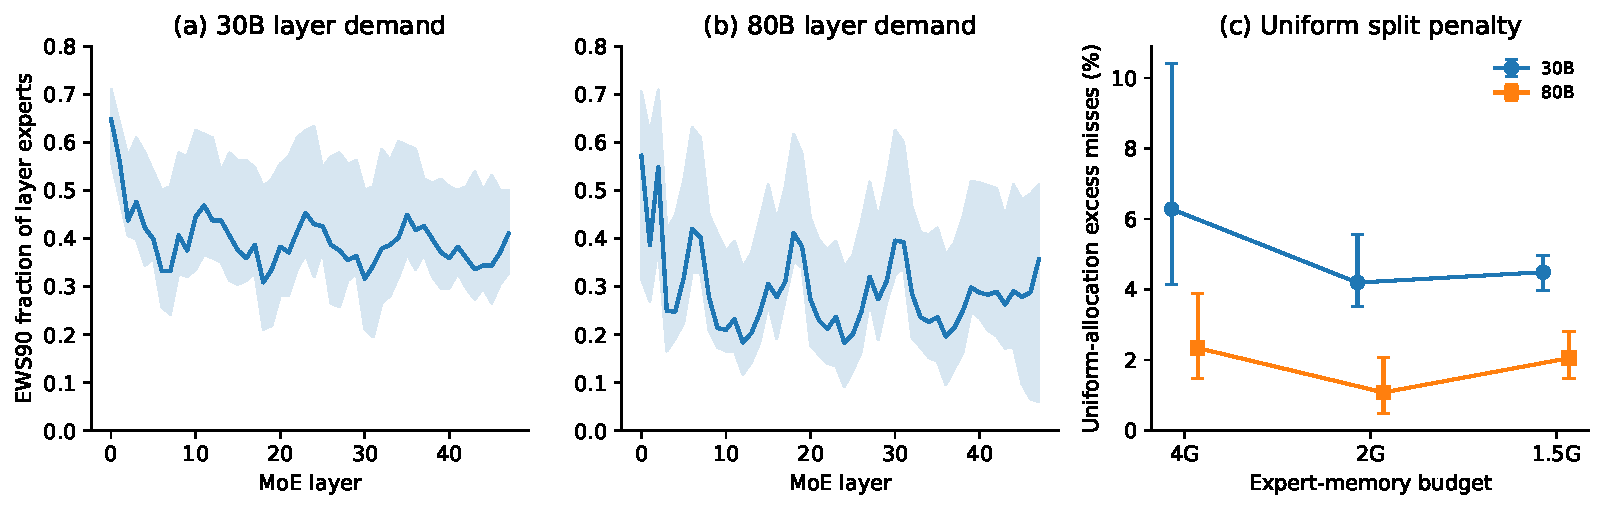
\includegraphics[width=\linewidth]{../experiments/EXP-007-router-characterization/figures/layer_heterogeneity_and_uniform_penalty.pdf}
    \caption{Layer demand is heterogeneous and uniform memory partitioning is measurably suboptimal. Panels (a) and (b) show the median per-layer EWS90 fraction across the 14 final in-sample workload/split cells for the 30B and 80B MoEs; shaded regions denote the full observed range. Layer-demand heterogeneity is present in both models, with per-cell EWS90 coefficients of variation spanning 0.085--0.248 for 30B and 0.162--0.455 for 80B. Panel (c) shows the median excess misses induced by a uniform per-layer memory split, with whiskers denoting the full observed range. The result establishes measurable allocation opportunity but does not imply that greater routing heterogeneity necessarily yields greater allocation benefit.}
    \label{fig:heterogeneity}
\end{figure}

The first question is whether a fixed expert-memory budget should be divided uniformly across MoE layers. If all layers exposed similar routed demand, a uniform partition would be a natural default. The EXP-007 characterization rejects that simplifying assumption within the evaluated traces.

Across the 14 final workload/split cells per model, global EWS90 fractions span approximately 0.327--0.554 for the 30B and 0.225--0.472 for the 80B. More importantly for allocation, the layer-by-layer working sets are not uniform within a trace. The coefficient of variation of per-layer EWS90 fractions ranges from 0.085 to 0.248 for the 30B and from 0.162 to 0.455 for the 80B. Figure~\ref{fig:heterogeneity}(a,b) shows that this heterogeneity is structured across depth rather than being a small perturbation around one common layer demand.

\subsection{The cost of a uniform layer split}

We quantify the allocation opportunity by replaying the same qualified routing trace under the same total memory budget while changing only the layer partition. Let $m_{\mathrm{uniform}}$ be the miss count obtained by splitting the budget uniformly across layers, and let $m_{\mathrm{static}}^{*}$ be the minimum miss count obtained by the in-sample static layer-allocation reference for that trace. We report the uniform-allocation excess
\begin{equation}
    E_{\mathrm{uniform}}
    =
    100\,
    \frac{m_{\mathrm{uniform}}-m_{\mathrm{static}}^{*}}
         {m_{\mathrm{static}}^{*}}
    \quad [\%].
    \label{eq:uniform-excess}
\end{equation}

The penalty is consistently larger for the 30B regime. Across the tested workload/split cells and budgets, the 30B uniform split incurs approximately 3.5--10.4\% excess misses, whereas the 80B incurs approximately 0.5--3.9\%. The effect is not explained by the 80B being more uniform. In fact, the 80B has the larger per-layer EWS spread, while exposing less exploitable inter-layer allocation opportunity.

The multi-turn workload makes this distinction concrete. Its 80B EWS90 fraction is lower than the 30B's, indicating more concentrated routing, yet its uniform-allocation penalty is substantially smaller. More generally, within each model there is an exploratory association between routing concentration and allocation opportunity, but that relationship does not transfer across models. Routing concentration is therefore not a model-agnostic proxy for the value of re-partitioning memory.

\begin{proposition}[Uniform layer allocation is suboptimal in the evaluated replay traces]
\label{prop:uniform-suboptimal}
For both evaluated MoE models, there exist qualified workload/split cells and memory budgets for which a non-uniform static allocation produces fewer misses than an equal per-layer split at the same global budget $M$.
\end{proposition}

\begin{proof}
EXP-007 replays identical qualified routing events at fixed $M$ while varying only the layer allocation. The measured excess in Eq.~\eqref{eq:uniform-excess} is strictly positive over the reported ranges, reaching 10.4\% for the 30B and 3.9\% for the 80B. Hence an equal split is not miss-minimal for those traces.
\end{proof}

The proposition is deliberately scoped. The comparator $m_{\mathrm{static}}^{*}$ is fitted to the same trace and therefore represents an in-sample memory-value reference, not an online policy and not an untouched out-of-sample result. The conclusion is that measurable layer-allocation opportunity exists; it does not establish that a particular adaptive controller can recover it in deployment.

\section{Allocation Helps, but Selection Dominates the Remaining Gap}
\label{sec:allocation-selection}

\begin{figure}[t]
    \centering
    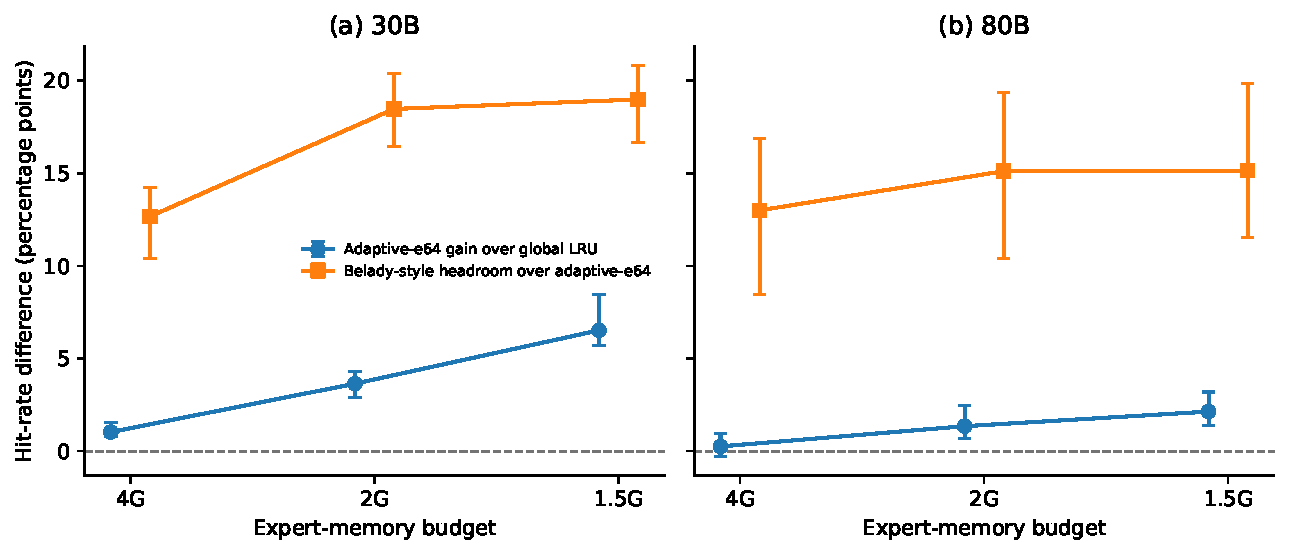
\includegraphics[width=\linewidth]{../experiments/EXP-007-router-characterization/figures/allocation_vs_selection.pdf}
    \caption{Allocation matters, but selection matters more. Median hit-rate improvement of \texttt{adaptive-e64} over global LRU and remaining Belady-style future-informed headroom across the 14 in-sample workload/split cells for each model and memory budget; whiskers show the full observed range. Layer-aware allocation becomes increasingly valuable under stronger memory pressure, especially for the 30B model. Nevertheless, the remaining future-informed selection headroom is substantially larger in every tested model/budget condition. The Belady-style reference is not an achievable online policy and is used only to quantify residual selection opportunity.}
    \label{fig:allocation-selection}
\end{figure}

Layer heterogeneity creates an allocation opportunity, but it does not tell us how much of the total cache-performance gap can be removed by moving capacity between layers. We therefore separate the gain attributable to the tested layer-aware controller from the remaining gain exposed by future-informed expert selection.

Let $h(P)$ denote the replay hit rate of policy $P$ on one trace and budget. Define
\begin{align}
    G_{\mathrm{alloc}}
    &=
    h(\texttt{adaptive-e64})-h(\mathrm{global\ LRU}),
    \label{eq:galloc}\\
    G_{\mathrm{select}}
    &=
    h(\mathrm{Belady})-h(\texttt{adaptive-e64}).
    \label{eq:gselect}
\end{align}
The first quantity asks how much is gained by the tested layer-aware allocation relative to conventional global recency. The second is not an achievable online gain: it measures how much expert-selection opportunity remains if future accesses are known.

\subsection{Allocation becomes more valuable under pressure}

For the 30B, \texttt{adaptive-e64} improves hit rate over global LRU by approximately 0.8--1.5 percentage points at 4\,GiB and 5.7--8.5 points at 1.5\,GiB across the 14 workload/split cells. For the 80B, the corresponding ranges are $-0.3$--$+0.9$ points at 4\,GiB and $+1.4$--$+3.2$ points at 1.5\,GiB. The direction is therefore clearest under stronger pressure, particularly for the 30B.

The gain should not be attributed entirely to rapid adaptation. At 1.5\,GiB, a fixed per-layer partition already captures most of the re-partitioning benefit; relative to that partition, the changing adaptive split adds only about 1.4--1.8 points on the 30B and 0.4--0.7 points on the 80B. Section~\ref{sec:workload-drift} tests the temporal mechanism directly.

Nor is \texttt{adaptive-e64} universally the best online-style replay policy. A 2Q alternative matches or exceeds it at several 80B points, mostly at 4\,GiB. The result of interest is therefore not that one controller dominates the policy space, but that layer-aware partitioning is useful in constrained regimes.

\subsection{The larger gap is within-layer selection}

Figure~\ref{fig:allocation-selection} shows a substantially larger residual gap to the Belady-style future-informed reference. Across the evaluated model/budget conditions, Belady remains approximately 8.5--20.8 percentage points above \texttt{adaptive-e64}. This residual is several times larger than the measured gain from re-splitting memory across layers.

\begin{proposition}[Selection headroom exceeds re-allocation headroom in the evaluated replay]
\label{prop:selection-headroom}
Within the EXP-007 replay abstraction, the remaining future-informed expert-selection headroom after \texttt{adaptive-e64} is larger than the layer-allocation gain recovered over global LRU across the tested model/budget conditions summarized in Figure~\ref{fig:allocation-selection}.
\end{proposition}

\begin{proof}
The ranges are separated in every model/budget group. For the 30B at 4, 2, and 1.5\,GiB, the maximum observed allocation gains are 1.542, 4.314, and 8.461 percentage points, while the minimum future-informed selection headrooms are 10.417, 16.432, and 16.677 points. For the 80B, the corresponding maxima are 0.936, 2.486, and 3.193 points, while the corresponding selection minima are 8.466, 10.394, and 11.552 points. Hence, in each of the six model/budget groups summarized in Figure~\ref{fig:allocation-selection}, even the largest observed re-allocation gain remains below the smallest observed future-informed selection headroom.
\end{proof}

The Belady comparison is intentionally an upper-reference calculation rather than a deployable algorithm. It does not imply that an online predictor can realize the full gap. It instead changes the optimization priority suggested by the data: once layer capacity is partitioned reasonably, the larger measured opportunity lies in deciding \emph{which} experts to retain, not merely in changing \emph{how much} memory each layer receives.

\section{Workload Drift Does Not Imply Useful Fast Adaptation}
\label{sec:workload-drift}

\begin{figure}[t]
    \centering
    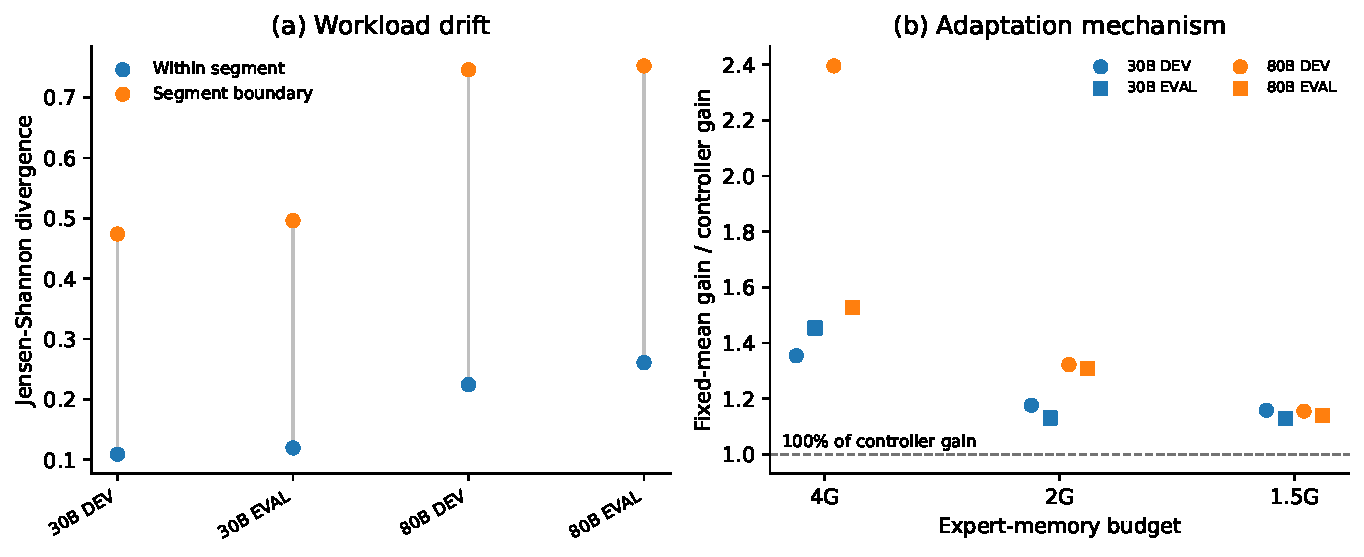
\includegraphics[width=\linewidth]{../experiments/EXP-023-workload-drift/figures/workload_drift_vs_adaptation.pdf}
    \caption{Workload drift does not imply useful fast adaptation. Panel (a) shows that Jensen--Shannon divergence between routing distributions is substantially larger across workload boundaries than within segments for both evaluated MoEs. Panel (b) compares the gain of a fixed allocation equal to the controller's mean allocation with the gain of the tested controller. The result confirms workload-dependent routing drift but falsifies the temporal mechanism of the current \texttt{adaptive-e64} controller; it does not establish that dynamic adaptation is ineffective in general.}
    \label{fig:workload-drift}
\end{figure}

The allocation results raise a natural temporal hypothesis: if workloads change, a controller that reacts to those changes may outperform a fixed layer partition. EXP-023 separates the two clauses of that hypothesis. The first clause---that routing distributions change at workload boundaries---is strongly supported descriptively. The second---that the current controller benefits from reacting rapidly to those changes---is falsified for \texttt{adaptive-e64}.

\subsection{Routing distributions move at workload boundaries}

The transition traces contain four segments with qualitatively different workloads. For each boundary and MoE layer, EXP-023 compares the last 64 counted decode steps of the outgoing segment with the first 64 of the incoming segment using Jensen--Shannon divergence. The reference is the JSD between adjacent non-overlapping 64-step windows within the corresponding segments.

\begin{table}[t]
    \centering
    \caption{Routing-distribution drift in the four transition traces. Ratios are medians of boundary JSD relative to the within-segment reference. This operationalization is retrospective and descriptive.}
    \label{tab:jsd-drift}
    \small
    \begin{tabular}{lrrr}
        \toprule
        Trace & Boundary JSD & Within JSD & Ratio \\
        \midrule
        30B DEV  & 0.4739 & 0.1091 & 3.810 \\
        30B EVAL & 0.4959 & 0.1196 & 4.022 \\
        80B DEV  & 0.7459 & 0.2246 & 3.381 \\
        80B EVAL & 0.7524 & 0.2608 & 2.839 \\
        \bottomrule
    \end{tabular}
\end{table}

Across all four traces, the median boundary divergence is 2.84--4.02 times the within-segment reference. Boundary JSD also exceeds the corresponding within-segment maximum in 96.5--100\% of layer-boundary rows. Workload transitions therefore induce large, repeatable changes in per-layer routing distributions.

This part of EXP-023 is deliberately not presented as a confirmatory hypothesis test: the JSD operationalization was fixed after the transition data already existed, and no $p$-value or success threshold was preregistered. Its role is descriptive characterization.

\subsection{The tested controller does not profit from fast reaction}

The temporal mechanism is tested independently of the JSD description. For each model, split, and budget, the analysis compares the controller's gain with a static allocation equal to the controller's \emph{mean} allocation over the trace. If the controller's advantage arose from timely movement of memory, averaging away that timing should remove a meaningful part of the gain.

It does not. The fixed mean allocation exceeds the controller's own gain in all 12 model/split/budget rows. The ratio of fixed-mean gain to controller gain ranges from 1.129 to 2.396. In addition, the reaction-lag cost relative to instantly switched segment allocations is negative in all 12 rows, ranging from $-1844$ to $-820$ misses. At individual boundaries, \texttt{adaptive-e64} has a lower signed 64-step departure from the new-segment steady state than the frozen split in only 11 of 36 comparisons; it is higher in 25 of 36.

\begin{proposition}[The temporal mechanism of \texttt{adaptive-e64} is falsified]
\label{prop:temporal-falsified}
For the four evaluated transition traces and three memory budgets, the observed gain of the current \texttt{adaptive-e64} controller cannot be attributed to beneficial rapid reaction to workload boundaries.
\end{proposition}

\begin{proof}
A timing-free comparator formed from the controller's own mean allocation matches or exceeds the controller gain in all 12 aggregate rows, while the measured reaction-lag comparison is unfavorable in all 12. Thus removing the temporal movement does not remove the gain; instead, the evidence attributes most or all of the benefit to the allocation partition itself rather than to fast transition response.
\end{proof}

The scope of Proposition~\ref{prop:temporal-falsified} is important. It does not imply that workloads are stationary, nor that dynamic adaptation is useless in general. The JSD measurements show the opposite: demand changes materially. The negative result applies to the current, untuned \texttt{adaptive-e64} temporal mechanism. A controller with better change detection, prediction, or faster actuation remains an open design direction.

\section{Hit Rate Is Not a Performance Model}
\label{sec:performance-model}

The replay results naturally use hit rate because they ask which accesses would have been served from resident memory. End-to-end performance, however, depends on the \emph{time} exposed by misses. Two complications prevent miss count from being a sufficient performance model: the runtime's hit counter has non-obvious semantics, and the time cost of a miss changes with I/O concurrency.

\begin{figure}[t]
    \centering
    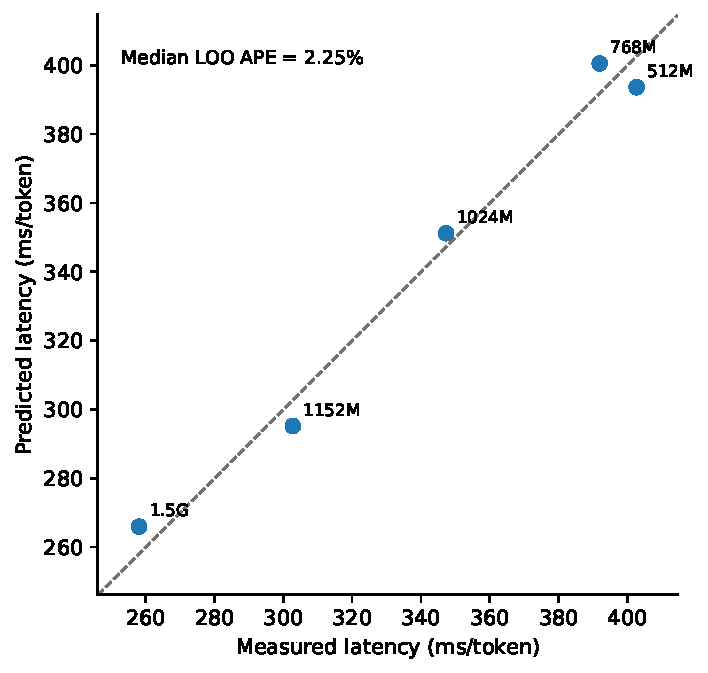
\includegraphics[width=0.72\linewidth]{../experiments/EXP-025-performance-model/figures/performance_model_predicted_vs_measured.pdf}
    \caption{Interpretable prediction of token latency. Measured versus leave-one-configuration-out predicted latency for the five preregistered 30B memory configurations. The dashed diagonal denotes perfect prediction. Median absolute percentage error is 2.25\%, below the preregistered 15\% criterion. The result supports the predictive usefulness of the latency decomposition over the tested configurations, without separately identifying every physical latency component.}
    \label{fig:performance-model}
\end{figure}

\subsection{Runtime hit accounting and expert reuse are different quantities}

In the evaluated expert store, the gate, up, and down nodes request the slices associated with an expert, but misses occur when the first node loads those slices; subsequent nodes re-pin them and hit. EXP-020 and EXP-021 establish this behavior record-for-record. Across the 252 qualified EXP-007 runs, the expert-level gate-slice miss rate is exactly three times the runtime-style miss rate.

Consequently, a runtime hit rate near 90\% does not imply a 90\% expert-level reuse rate. For example, on qualified 30B coding runs the workload-only expert-level hit rates are 70.60\%, 49.75\%, and 41.46\% at 4, 2, and 1.5\,GiB, while the corresponding runtime-style rates are 90.2\%, 83.2\%, and 80.5\%. The distinction is mechanical rather than statistical and is preserved throughout this paper.

This also separates the runtime metrics from the replay's whole-expert event metric. A single generic ``hit rate'' would conflate three different questions: whether the runtime reused a slice, whether the routed expert was already available at the gate, and whether all slices required by an event were resident together.

\subsection{Misses do not have a constant wall-clock cost}

The storage path is asynchronous. As pressure increases, more misses can create more reads in flight, increasing queue depth and improving I/O overlap. Consequently, the wall-clock cost of an additional miss need not be constant across configurations: a policy that prevents one additional miss does not necessarily save a fixed amount of time.

This is why the performance question cannot be reduced to
\[
    T_{\mathrm{token}}
    \propto
    \text{misses/token}.
\]
The quantity of interest is the \emph{unhidden} I/O time after concurrency and overlap, together with compute and other runtime costs.

\subsection{Leave-one-configuration-out latency prediction}

EXP-025 tests the latency model introduced in Eq.~\eqref{eq:latency-model} on five preregistered 30B memory configurations. For each held-out budget, the non-negative coefficients are fitted on the other four configurations and then used to predict the held-out ms/token. Table~\ref{tab:loo-predictions} reports the resulting predictions.

\begin{table}[t]
    \centering
    \caption{EXP-025 leave-one-configuration-out predictions. APE is absolute percentage error.}
    \label{tab:loo-predictions}
    \small
    \begin{tabular}{lrrr}
        \toprule
        Budget & Measured ms/token & Predicted ms/token & APE (\%) \\
        \midrule
        1.5G  & 258.115 & 265.927 & 3.027 \\
        1152M & 302.794 & 295.161 & 2.521 \\
        1024M & 347.339 & 351.194 & 1.110 \\
        768M  & 391.974 & 400.530 & 2.183 \\
        512M  & 402.710 & 393.630 & 2.255 \\
        \bottomrule
    \end{tabular}
\end{table}

The median held-out absolute percentage error is
\begin{equation}
    \mathrm{median\ APE}
    =
    2.2546885\%,
    \label{eq:median-ape}
\end{equation}
well below the preregistered 15\% criterion. The primary predictive hypothesis is therefore supported for this 30B configuration family.

\begin{proposition}[The latency decomposition is predictive on the preregistered 30B test]
\label{prop:latency-predictive}
For the five EXP-025 memory configurations, the decomposition in Eq.~\eqref{eq:latency-model} predicts held-out token latency with median absolute percentage error below the preregistered 15\% threshold.
\end{proposition}

\begin{proof}
The five leave-one-configuration-out errors in Table~\ref{tab:loo-predictions} have median 2.2546885\%, which is strictly below 15\%.
\end{proof}

\subsection{Predictive decomposition is not component identification}

The success of Proposition~\ref{prop:latency-predictive} should not be read as a causal identification of every term. In the five primary configurations, \texttt{nodes\_per\_token} is constant at 142.875. The fitted intercept-like compute term and the synchronization term are therefore collinear. The fitted synchronization coefficient being effectively zero does \emph{not} establish that physical synchronization cost is zero.

Likewise, reconstructed queue depths retain upper-bound status where completion timestamps are bounded, and tracing overhead is not independently bounded at or below 1.5\,GiB. EXP-025 supports the usefulness of a time-based decomposition over the tested range; it does not establish that its coefficients are unique physical constants. The broader conclusion is narrower but important: hit rate is useful for describing reuse, yet insufficient by itself to predict performance.

\section{Pressure Regimes Are Not Universal Residency Thresholds}
\label{sec:pressure-regimes}

\begin{figure}[t]
    \centering
    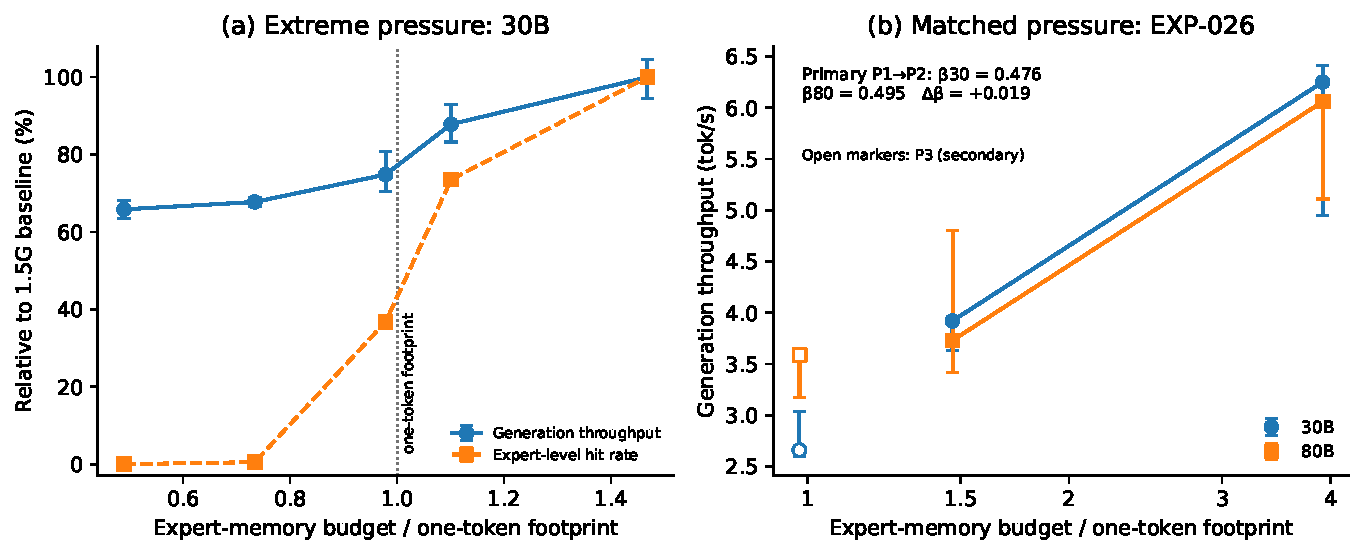
\includegraphics[width=\linewidth]{../experiments/EXP-026-30b-vs-80b-regimes/figures/cross_regime_synthesis.pdf}
    \caption{Reuse transitions and performance regimes are not universal residency thresholds. Panel (a) shows the 30B extreme-pressure result normalized to the 1.5\,GiB baseline: expert-level reuse collapses substantially faster than generation throughput, and execution continues below the one-token expert footprint. Panel (b) shows the matched-pressure comparison: the preregistered P1$\rightarrow$P2 pressure-response exponents are $\beta_{30}=0.476$ and $\beta_{80}=0.495$ ($\Delta\beta=+0.019$), so the models are not distinguished by the primary explanandum. Open markers show the secondary P3 condition.}
    \label{fig:pressure-regimes}
\end{figure}

The preceding sections show that cache capacity, hit rate, and layer allocation each capture only part of the system. We next ask whether a simple normalized capacity scale can nevertheless define a universal operating regime. Two experiments answer different parts of that question: EXP-022 pushes one model through extreme pressure, while EXP-026 compares both models at matched $M/F$ on the current runtime.

\subsection{Reuse can collapse before execution does}

Table~\ref{tab:extreme-pressure} summarizes the 30B primary arm of EXP-022. All 15 untraced performance launches and all 10 diagnostic launches completed validly down to 512\,MiB.

\begin{table}[t]
    \centering
    \caption{30B extreme-pressure means. The hit rate is the diagnostic workload gate-slice expert-level rate; throughput comes from separate untraced performance launches.}
    \label{tab:extreme-pressure}
    \small
    \begin{tabular}{lrrr}
        \toprule
        Budget & $M/F$ & Throughput (tok/s) & Expert-level hit (\%) \\
        \midrule
        1.5G  & 1.468 & 4.00 & 44.01 \\
        1152M & 1.101 & 3.51 & 32.37 \\
        1024M & 0.979 & 2.99 & 16.19 \\
        768M  & 0.734 & 2.71 & 0.232 \\
        512M  & 0.489 & 2.63 & 0.000 \\
        \bottomrule
    \end{tabular}
\end{table}

The two response variables separate sharply below the footprint. At $M/F=0.489$, the diagnostic expert-level hit rate has fallen to zero, yet throughput remains 2.63\,tok/s, approximately 65.8\% of the 1.5\,GiB baseline. At 768\,MiB ($0.734F$), reuse is already only 0.232\% while throughput remains 2.71\,tok/s.

Thus the one-token footprint marks neither a hard completion boundary nor a point at which useful throughput vanishes. It is more consistent with a transition scale for recency-based reuse under this workload. The preregistered historical H-5 falsifier at 30B/768\,MiB required an expert-level hit rate above 30\%; the observed mean was 0.2322\%. The historical prediction was therefore \emph{not falsified by this test}, but the experiment remains formally inconclusive because no positive support threshold had been specified.

The exploratory 80B arm reinforces the separation between low reuse and hard infeasibility. At 512\,MiB, two performance replicas completed in a degraded state while one encountered \nolinkurl{STORE_RESIDENCY_ABORT}. The mixed outcome does not establish 512\,MiB as an intrinsic physical lower bound for the model.

\begin{proposition}[The one-token footprint is not a hard execution threshold in the 30B extreme-pressure workload]
\label{prop:not-hard-threshold}
For the evaluated 30B runtime and workload, valid generation continues at expert-memory budgets strictly below the one-token footprint $F$.
\end{proposition}

\begin{proof}
The 30B footprint is approximately 1.0217\,GiB. Valid performance launches complete at both 768\,MiB ($0.734F$) and 512\,MiB ($0.489F$), with mean throughputs of 2.71 and 2.63\,tok/s. Therefore $M=F$ is not a necessary condition for execution in this workload.
\end{proof}

\subsection{The historical cross-model regime difference does not reproduce at matched pressure}

Historical sessions had suggested different sublinear pressure-response slopes for the two models, but those comparisons covered different normalized pressure regions and earlier binaries. EXP-026 prospectively removes two major confounds: the primary points are matched by $M/F$, and both models are measured on the current runtime within one session. Both models keep four generation threads, the thread condition of the historical comparison.

For the primary P1$\rightarrow$P2 comparison, the observed median throughputs are:

\begin{table}[t]
    \centering
    \caption{EXP-026 primary matched-pressure performance. Parentheses give the observed range over three valid launches.}
    \label{tab:exp026-primary}
    \small
    \begin{tabular}{lrr}
        \toprule
        & P1 & P2 \\
        \midrule
        30B & 6.25\ (4.95--6.41) & 3.92\ (3.63--3.96) \\
        80B & 6.06\ (5.11--6.06) & 3.73\ (3.42--4.80) \\
        \bottomrule
    \end{tabular}
\end{table}

The preregistered pressure-response exponents are
\begin{equation}
    \beta_{30}=0.4756076,
    \qquad
    \beta_{80}=0.4947870,
    \qquad
    \Delta\beta=+0.0191794 .
    \label{eq:exp026-beta}
\end{equation}
Their launch-pair envelopes are
\[
    \beta_{30}\in[0.2275,\,0.5797],
    \qquad
    \beta_{80}\in[0.0638,\,0.5833],
\]
which overlap strongly. Under the frozen decision rule, the primary explanandum is therefore \textbf{not distinguished}. The historical flatter-80B regime does not reproduce over the matched-$F$ P1--P2 region on the current runtime.

This is a non-reproduction, not a retrospective invalidation. The earlier regimes were measured over different $M/F$ regions on earlier binaries and remain valid descriptions of those sessions. The matched-pressure result is consistent with the possibility that normalization or pressure region contributed to the historical contrast, but it does not establish that either factor \emph{caused} it.

\subsection{Mechanism attribution remains inconclusive}

EXP-026 also collected traced diagnostic measurements intended to discriminate candidate explanations if the primary cross-model difference reproduced. Those diagnostic slopes do not agree with the untraced primary result:
\[
    \beta_{30,\mathrm{traced}}=0.4960,
    \qquad
    \beta_{80,\mathrm{traced}}=0.2266,
    \qquad
    \Delta\beta_{\mathrm{traced}}=-0.2694.
\]
The sign of the traced difference is opposite to the primary $\Delta\beta$, so the preregistered agreement gate fails. Consequently, the candidate mechanisms---routing concentration, slice-size/queue-depth effects, bookkeeping, and compute---are all \emph{not evaluable} against the primary explanandum. The EXP-026 lifecycle status is therefore INCONCLUSIVE even though the primary non-reproduction itself is informative.

The secondary P3 condition is reported descriptively in Figure~\ref{fig:pressure-regimes}. Its median throughput is 2.66\,tok/s for the 30B and 3.59\,tok/s for the 80B at $M/F\approx0.979$. This endpoint should not be used to replace the frozen P1$\rightarrow$P2 decision.

Taken together, EXP-022 and EXP-026 rule out a simple universal-threshold interpretation. Below $F$, reuse can collapse while execution continues; at matched pressure above $F$, the historical cross-model slope difference need not reproduce. Resident fraction and one-token footprint are useful coordinates, but neither is a complete performance law.

\section{Discussion}
\label{sec:discussion}

The experiments in Sections~\ref{sec:heterogeneity}--\ref{sec:pressure-regimes} point to a systems problem that is broader than conventional cache sizing. Under a hard DRAM ceiling, expert streaming couples three decisions: how capacity is partitioned across layers, which experts are retained within that capacity, and how the resulting misses are scheduled and overlapped with computation. The data do not support reducing this interaction to resident fraction, a single hit-rate metric, or one universal pressure threshold.

\subsection{Expert residency is a joint allocation-and-retention problem}

The first implication is structural. Layer working sets are heterogeneous, and a uniform split is measurably suboptimal in the evaluated replay traces. This establishes that memory placement across layers has value. Yet the residual future-informed selection headroom remains larger than the gain recovered by the tested re-allocation mechanism in every model/budget group summarized in Figure~\ref{fig:allocation-selection}. The resulting design priority is therefore not ``find the optimal layer split'' in isolation. A practical system must coordinate layer allocation with the policy that decides which experts occupy each layer's capacity.

This distinction also explains why routing concentration alone is not a sufficient allocation signal. The 80B exposes larger per-layer EWS variability than the 30B while yielding a smaller uniform-allocation penalty. More heterogeneous demand does not automatically imply more value from re-partitioning memory. A controller therefore needs a memory-value objective that is closer to avoided time cost than to routing concentration by itself.

\subsection{Selection quality is the larger measured opportunity}

The Belady-style reference is deliberately unattainable online, but its role is informative: it measures the amount of replay headroom left after the tested layer-aware policy. The fact that this gap remains 8.5--20.8 percentage points across the evaluated model/budget groups means that a substantial part of the remaining opportunity lies inside the layer partitions.

This suggests a progression for future systems. First, avoid obviously poor global or uniform allocation under strong pressure. Second, invest in expert-level prediction and retention mechanisms that anticipate near-future demand. Third, evaluate those mechanisms using wall-clock value rather than hit rate alone. Candidate approaches include short-horizon reuse prediction, cost-aware admission, asymmetric eviction, and prefetching, but the present experiments do not compare such algorithms and therefore do not establish which is preferable.

\subsection{Workload drift requires prediction, not merely reaction}

EXP-023 separates the existence of non-stationarity from the usefulness of the tested controller's temporal response. Routing distributions change strongly at workload boundaries, yet the current \texttt{adaptive-e64} controller obtains no demonstrated benefit from reacting rapidly to those boundaries. A fixed allocation equal to the controller's mean allocation matches or exceeds the controller gain in every aggregate transition condition.

The important conclusion is not that adaptation is unnecessary. Rather, \emph{reactivity without an effective temporal mechanism is insufficient}. A useful adaptive controller must detect a change early enough, estimate whether the new regime will persist long enough to repay movement costs, and move capacity in a direction that improves future retention. In this sense the failed temporal mechanism narrows the design problem: the useful signal exists, but the tested way of exploiting it does not.

The transition experiment also motivates a distinction between \emph{partition adaptation} and \emph{retention adaptation}. A workload boundary may alter which experts are valuable without requiring a large change in the layer-level memory split. Future controllers should therefore test both timescales separately rather than assuming that routing drift implies rapid movement of capacity between layers.

\subsection{Performance objectives should be expressed in time}

The performance-model experiment provides a second design implication. Misses are not equal-cost events. Their exposed cost depends on queue depth, read overlap, slice size, and the amount of I/O hidden behind computation. This is why expert-level reuse and runtime-style hit accounting can both be useful yet remain insufficient as direct optimization objectives.

A practical controller should ideally estimate the marginal latency value of keeping or fetching an expert:
\begin{equation}
    V(e,l,t)
    \approx
    \Pr(\text{reuse of } e)
    \times
    \mathbb{E}[\text{unhidden I/O saved}]
    -
    \text{opportunity cost of resident bytes}.
    \label{eq:memory-value}
\end{equation}
Equation~\eqref{eq:memory-value} is a design abstraction rather than a fitted model in this paper. Its purpose is to make explicit what the experiments imply: the relevant benefit is avoided exposed time, not avoided misses in the abstract.

The success of the EXP-025 latency decomposition strengthens this view. A small set of interpretable time components predicts the five held-out 30B configurations with 2.25\% median absolute percentage error, while simple miss count is not a sufficient elapsed-time model. The fitted coefficients should not be read as uniquely identified physical constants, but the predictive result supports a time-based objective for future policy work.

\subsection{Normalized pressure is useful but not universal}

The one-token footprint $F$ provides a useful physical scale because it relates memory capacity to the routed expert demand of one token. It is particularly helpful when the two models have very different total expert-store sizes. Nevertheless, the extreme-pressure and matched-pressure experiments show why $M/F$ should be treated as a coordinate rather than a universal law.

For the 30B, execution remains valid well below $F$ even after diagnostic expert-level reuse has collapsed to approximately zero. Conversely, matching $M/F$ across the two models does not reproduce the historical cross-model pressure-response difference on the current runtime. These observations rule out two simple interpretations: $F$ is not a hard feasibility threshold in the evaluated workload, and matched $M/F$ does not by itself guarantee a model-independent throughput response.

The more defensible interpretation is that $F$ identifies a pressure region in which retention becomes difficult, while the realized performance curve still depends on model architecture, expert sizes, routing, binary behavior, concurrency, and the workload. The present data do not identify a single causal variable that explains the historical 30B/80B difference.

\subsection{Negative results constrain the design space}

Two preregistered mechanism questions do not produce positive confirmations. The temporal mechanism of \texttt{adaptive-e64} is falsified in EXP-023, and the historical cross-model slope difference is not distinguished in the matched-pressure primary test of EXP-026. These outcomes are useful precisely because the artifact retains them without redefining the hypothesis after observing the data.

This discipline matters for systems work, where many plausible explanations can be constructed retrospectively from the same performance curve. The experiment ledger, frozen decision rules, replay validation, and explicit distinction between measured, derived, descriptive, supported, falsified, and inconclusive quantities reduce that flexibility. The resulting narrative is less universal, but it is more informative about what a future system must still demonstrate.

\subsection{Implications for an online expert-streaming runtime}

Taken together, the evidence suggests four requirements for a stronger online runtime:
\begin{enumerate}
    \item \textbf{Layer-aware capacity management.} Uniform partitioning leaves measurable reuse on the table under pressure.
    \item \textbf{Predictive expert retention.} The larger residual replay headroom lies in within-layer expert selection.
    \item \textbf{Cost-aware I/O decisions.} Policies should value avoided \emph{unhidden} latency rather than assuming a constant cost per miss.
    \item \textbf{Evidence-based temporal control.} Adaptation should move memory only when detected regime changes are expected to persist long enough to repay the change.
\end{enumerate}

Argine does not yet implement all four as one production controller. The contribution of the present study is to separate these requirements experimentally and to show where simpler abstractions fail.

\section{Limitations}
\label{sec:limitations}

The scope of the results is intentionally narrower than the general problem of MoE memory management.

\paragraph{One hardware platform.}
All end-to-end measurements were collected on one Windows~11 consumer system with an Intel Core i5-1340P, 16\,GB of RAM, NVMe storage, and CPU-only execution. The results therefore do not establish transfer to servers, different storage devices, NUMA systems, GPUs, unified memory, CXL, or heterogeneous CPU--GPU inference.

\paragraph{Two model regimes.}
The study evaluates two quantized MoE models. They differ simultaneously in total parameter count, routed-expert count, expert sizes, quantization, architecture, and shared-expert structure. Cross-model observations should therefore be interpreted as comparisons of two concrete regimes, not as a scaling law over model size.

\paragraph{Binary provenance matters.}
The research campaign spans more than one validated runtime binary. Historical findings remain descriptions of the sessions in which they were measured, while later confirmatory experiments use the current research runtime. This design preserves evidence but limits direct pooling of timings across the full campaign.

\paragraph{Replay is not end-to-end execution.}
The allocation and selection comparisons rely on event-atomic replay validated against the expert store under qualified conditions. Replay is appropriate for counterfactual cache-policy comparisons, but it does not reproduce every timing effect of a live runtime. In particular, replay hit-rate improvements should not be interpreted directly as equivalent throughput improvements.

\paragraph{The future-informed reference is unattainable online.}
The Belady-style policy uses future information. It is included only to quantify residual selection opportunity. Its headroom is not a realizable performance claim and may overstate what a causal online predictor can recover.

\paragraph{The tested adaptive controller is narrow.}
The negative temporal result applies to the current, untuned \texttt{adaptive-e64} mechanism and the evaluated transition traces. It does not test all adaptive controllers, prediction horizons, change detectors, or actuation strategies. Dynamic adaptation as a general approach remains open.

\paragraph{The latency model is primarily a 30B result.}
EXP-025 validates the interpretable time decomposition on five preregistered 30B memory configurations. The median leave-one-configuration-out error is low, but the study does not establish the same predictive accuracy for the 80B, other binaries, other machines, or other workload families. In addition, the constant nodes/token term makes the fitted compute/intercept and synchronization contributions collinear.

\paragraph{Tracing overhead is not universally bounded.}
EXP-024 places the 95\% confidence interval for tracing overhead entirely below 2\% at 4\,GiB, but the 1.5\,GiB result is inconclusive. Traced mechanism data at stronger pressure should therefore not be treated as interchangeable with untraced performance measurements.

\paragraph{Extreme-pressure feasibility is workload-specific.}
The observation that the 30B continues to execute below its one-token expert footprint applies to the tested prompt, runtime, and shard configuration. It does not prove that every workload or every model can execute at the same $M/F$, nor does the exploratory mixed 80B outcome at 512\,MiB define a universal lower bound.

\paragraph{The matched-pressure mechanism test remains inconclusive.}
In EXP-026 the primary untraced slopes are not distinguished, while the traced slopes disagree in sign with the primary difference. The preregistered agreement gate therefore fails, leaving the candidate explanations not evaluable. The experiment narrows the historical observation but does not identify its cause.

\paragraph{No final universal policy claim.}
Several replay analyses are in-sample memory-value studies, and the project does not contain an untouched final holdout covering every policy question. The evidence supports specific structural conclusions---for example, that uniform allocation can be suboptimal and that hit rate alone is insufficient---but does not establish a universally optimal online memory manager.

These limitations are also the main axes along which the results should be replicated: additional MoE architectures, independent machines and storage devices, live implementations of predictive retention and adaptive allocation, and prospective workload holdouts.

\section{Related Work}
\label{sec:related-work}

Recent surveys organize MoE inference optimization across model-, system-, and hardware-level techniques~\cite{liu2026survey}. Argine is closest to work on memory-constrained inference, expert offloading, caching, and prediction, but differs in experimental emphasis: rather than proposing a single offloading policy, it characterizes the allocation, retention, metric, and pressure-regime assumptions on which such policies depend.

\subsection{Sparse MoE architectures and distributed inference}

Modern sparse MoE systems build on sparsely gated conditional computation, in which a router activates only a small subset of a much larger expert pool~\cite{shazeer2017sparsely}. GShard demonstrated large-scale conditional computation with automatic sharding~\cite{lepikhin2020gshard}, while Switch Transformers simplified sparse routing and scaled MoE models to trillion-parameter regimes~\cite{fedus2022switch}. These works establish the architectural motivation for large expert pools whose total parameter footprint can greatly exceed the parameters active for one token.

Systems such as DeepSpeed-MoE and Tutel primarily address efficient MoE execution at data-center scale through compression, parallelism, communication optimization, and adaptive distributed execution~\cite{rajbhandari2022deepspeedmoe,hwang2023tutel}. Argine studies a complementary regime: a single consumer CPU with a hard DRAM budget, where expert weights are streamed from NVMe rather than distributed across an accelerator cluster. The resulting bottleneck is not all-to-all communication between expert-parallel workers, but which expert weights occupy a small resident pool and how non-resident demand becomes exposed storage time.

\subsection{Memory-constrained LLM inference}

Memory pressure has also motivated dense-model inference systems that span GPU memory, host memory, and storage. FlexGen searches for tensor placement and access schedules across GPU, CPU, and disk to maximize throughput under limited accelerator memory~\cite{sheng2023flexgen}. PagedAttention and vLLM instead address dynamic KV-cache allocation using paging-inspired memory management~\cite{kwon2023pagedattention}. These systems show that memory placement and movement policy can be first-order inference concerns even outside MoE.

Argine differs in both granularity and objective. Its managed objects are sparsely requested expert-weight slices, while non-expert weights remain outside the expert-memory budget. The central question is therefore not a static placement of full layers or KV blocks, but the interaction between router-driven demand, layer allocation, expert retention, and asynchronous storage reads at batch-one generation.

\subsection{Expert offloading and heterogeneous execution}

A growing line of work exploits MoE sparsity directly. Eliseev and Mazur showed that expert-aware offloading can make models such as Mixtral practical on limited consumer hardware~\cite{eliseev2023offloading}. EdgeMoE partitions MoE models across an edge-device storage hierarchy and combines expert prediction with bit-width adaptation~\cite{yi2023edgemoe}. MoE-Infinity uses request-level activation traces to drive a sparsity-aware expert cache, prefetching, and replacement on personal machines~\cite{xue2025moeinfinity}. These systems are particularly close to Argine in recognizing that only a subset of experts should occupy fast memory at a time.

Other systems reduce transfer cost by changing where or how missed experts execute. Fiddler orchestrates CPU and GPU execution to reduce CPU--GPU movement when GPU memory is insufficient~\cite{kamahori2025fiddler}. AdapMoE combines adaptive expert gating and expert management for efficient inference~\cite{zhong2024adapmoe}. Klotski uses expert-aware multi-batch pipelining and correlation-aware prefetching to overlap expert I/O with computation~\cite{fang2025klotski}. MoE-APEX further uses adaptive precision for cache-miss experts together with prefetching and cost-aware caching~\cite{tang2026moeapex}.

Argine does not compete with these systems as an end-to-end GPU offloading engine. Its contribution is orthogonal: it measures how much opportunity is attributable to layer allocation versus within-layer selection, validates replay semantics against the runtime, separates reuse metrics from elapsed-time prediction, and tests whether apparently natural temporal and normalized-pressure explanations survive direct experiments. These questions matter to offloading systems because a high hit rate, an adaptive partition, or a normalized memory ratio is useful only insofar as it predicts or reduces exposed latency.

\subsection{Expert prediction, prefetching, and cache-aware routing}

Expert prediction attempts to hide transfer latency by learning or exploiting structure in router decisions. Cache-Conditional Experts modifies routing itself to favor cached experts on memory-constrained mobile devices~\cite{skliar2024cacheconditional}. Local-routing-consistency analysis shows that the amount of exploitable temporal locality varies substantially across MoE architectures, cautioning against assuming that all models are equally cacheable~\cite{liang2025routingconsistency}. Pre-attention expert prediction uses same-layer pre-attention activations to forecast routing early enough for prefetching~\cite{zhu2025preattention}. Fate uses cross-layer gate information and a shallow-favoring cache policy for edge inference~\cite{fang2026fate}, while DoMoE exploits domain locality to narrow semantic expert prediction~\cite{mu2026domoe}.

These approaches motivate the large future-informed selection gap observed in Section~\ref{sec:allocation-selection}: there is substantial value in predicting \emph{which} experts will be needed, not only in deciding how much memory each layer receives. Argine's Belady-style reference is intentionally not a prediction algorithm. Following the classical role of optimal offline replacement~\cite{belady1966replacement}, it serves as a future-informed reference against which the residual retention opportunity can be measured. The paper therefore does not claim that the measured headroom is online-achievable.

\subsection{Dynamic allocation and online serving}

Dynamic resource allocation appears at multiple levels of MoE systems. Distributed serving can reassign accelerator resources as expert popularity changes; recent theoretical work formalizes this as an online MoE-serving problem with reconfiguration cost~\cite{huang2026moeserving}. Argine considers a different resource: bytes of a fixed local expert-memory pool. Nevertheless, both settings expose the same broad tension between reacting to a changing demand distribution and paying the cost of changing the allocation.

The transition results in Section~\ref{sec:workload-drift} add an empirical qualification to this literature. Strong routing drift is observable, but it does not follow that a reactive controller is useful: the tested \texttt{adaptive-e64} temporal mechanism is outperformed by a timing-free mean allocation in the evaluated transitions. This distinguishes the existence of non-stationarity from the value of a particular adaptation rule and motivates future controllers that evaluate movement in terms of predicted time savings rather than change detection alone.

\subsection{Position of this work}

The closest prior systems generally optimize one or more of expert prediction, caching, prefetching, quantization, heterogeneous execution, or I/O overlap. Argine instead treats the expert store as an experimental object and asks which abstractions remain valid under a hard memory ceiling. Its main differences are: (i) CPU-only NVMe-to-DRAM expert streaming rather than host-to-GPU expert offload; (ii) explicit separation of layer allocation from within-layer retention; (iii) event-atomic replay validated against runtime behavior; (iv) empirical separation of runtime hit semantics, expert-level reuse, and time cost; (v) preregistered negative tests of temporal adaptation and cross-model pressure explanations; and (vi) extreme-pressure measurements below the one-token expert footprint.

Accordingly, the paper should be read as a characterization and systems-analysis complement to expert-offloading engines, not as a replacement for them. Its results identify assumptions that future caching and prefetching mechanisms can use as design constraints and, equally importantly, assumptions they should not take for granted.

\section{Conclusion}
\label{sec:conclusion}

This paper examined expert streaming for mixture-of-experts inference under a hard DRAM budget. The experiments show that the problem is not adequately described by resident fraction or conventional hit rate alone.

Layer demand is heterogeneous, and uniform per-layer partitioning produces measurable excess misses. Layer-aware allocation helps increasingly under strong pressure, but the larger measured replay opportunity remains in future-informed expert selection. Routing distributions change sharply at workload boundaries, yet the current \texttt{adaptive-e64} controller does not obtain its gain from rapid temporal reaction. At the performance level, miss count is not a sufficient time model: an interpretable decomposition predicts the preregistered 30B token latencies with 2.25\% median leave-one-configuration-out error while preserving the distinction between reuse and exposed I/O cost. Finally, the one-token expert footprint is not a hard execution threshold in the evaluated extreme-pressure workload, and the historical 30B/80B pressure-regime difference does not reproduce in the matched-$M/F$ primary comparison on the current runtime.

The resulting systems view is therefore a coupled one. Under hard memory constraints, expert residency should be treated as a joint allocation-and-retention problem whose value is mediated by selection quality, I/O concurrency, and workload dynamics. The evidence does not establish a universal optimal policy. It instead identifies where simple abstractions fail and where the remaining optimization headroom lies: predictive expert selection, cost-aware I/O management, and temporal control that demonstrates value beyond a good static partition.


\section*{Artifact Availability}

The research artifact underlying the results reported in this paper is publicly available at \url{https://github.com/sennape/Argine2}. The frozen research-evidence snapshot is release \texttt{v0.2.0}, corresponding to commit \texttt{8ed817dc05a7db5a7e7e22138fa4d75bfc6c5e17}. The repository contains the runtime, research instrumentation, experiment registry, processed evidence, frozen protocols, analysis artifacts, tests, and reproducibility instructions used to support the reported claims.

The larger external raw trace corpus is not distributed through the Git repository. File-level SHA-256 metadata and experiment-level summaries are provided in \texttt{data/external\_raw\_manifest.csv} and \texttt{data/external\_raw\_summary.json}, respectively. Historical provenance, including the relationship between the clean public snapshot and retained pre-publication provenance identifiers, as well as platform-specific workload-byte conventions, is documented in \texttt{REPRODUCING.md}.

Release \texttt{v0.2.0} is retained as the immutable research-evidence snapshot. Subsequent paper-only editorial corrections do not modify the frozen measurements, experimental protocols, decision rules, or reported experimental outcomes.

\bibliographystyle{unsrt}
\bibliography{references}

\end{document}

